\section{Busca Binária}

\begin{frame}[fragile]\frametitle{Busca binária}

    \begin{itemize}
        \item A busca binária utiliza o paradigma de divisão e conquista para, a cada etapa de
            uma busca, descartar uma parte significativa das possíveis localizações do elemento a
            ser identificado

        \item Para tal, é necessário que os elementos estejam dispostos em uma determinada 
            ordenação

%        \item Também é desejável, mas não estritamente necessário, que o acesso aleatório aos
%            elementos seja eficiente

        \item A etapa de divisão escolhe o elemento $m$ que esteja na posição central, ou próximo a
            ela, quando os elementos estão dispostos de acordo com a ordenação

        \item O conjunto de elemento então é dividido em 3 conjuntos disjuntos: os elementos que
            ficaram à esquerda de $m$ ($L$), um conjunto unitário com o próprio $m$ e os elementos
            que estão à direita de $m$ ($R$)
    \end{itemize}

\end{frame}

\begin{frame}[fragile]\frametitle{Busca binária}

    \begin{itemize}
        \item A etapa de conquista acontece neste conjunto unitário

        \item Caso o elemento desejado seja $m$, o algoritmo termina

        \item Caso não seja, a busca continua em apenas um dos conjuntos $L$ ou $R$, a depender
            da relação do elemento procurado com $m$

        \item Neste algoritmo, não há uma etapa de fusão

		\item A ordem de complexidade da busca binária é $O(\log N)$, desde que o acesso aleatório
            seja feito em $O(1)$
    \end{itemize}

\end{frame}

\begin{frame}[fragile]\frametitle{Busca binária em vetores}

	\begin{itemize}
		\item A busca binária se vale da ordenação de um vetor de $N$ elementos para acelerar o 
        processo de busca

		\item Assuma que o vetor esteja em ordem crescente

        \item A busca binária identifica, primeiramente, o elemento $m$ que está na posição
            central do intervalo $[a, b]$ ($m = (a + b)/2$) e o elemento $x$ a ser localizado

        \item Se $x = m$, a busca retorna verdadeiro; caso contrário, ela compara os valores de $x$         e $m$

        \item Se $x < m$, a busca reinicia no intervalo à esquerda de $m$ ($[a, m - 1]$); 
        se $x > m$, a busca continua no subvetor à direita da $m$ ($[m + 1, b]$)

        \item Se $b < a$, a busca retorna falso
	\end{itemize}
 
\end{frame}  

\begin{frame}[fragile]{Visualização da busca binária}

    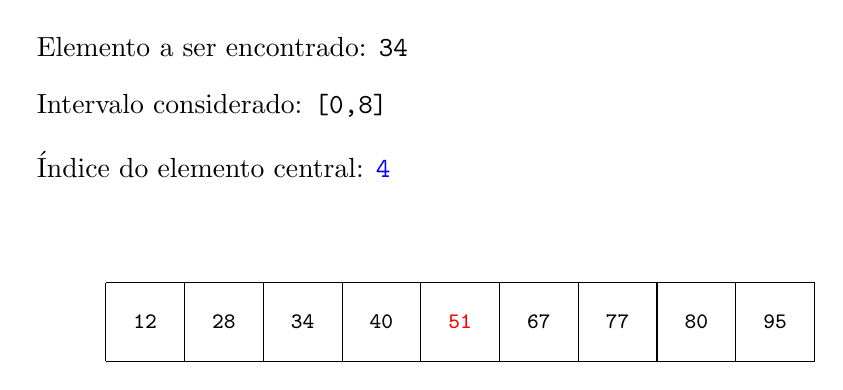
\begin{tikzpicture}
        \node[anchor=west] at (0, 4) {Elemento a ser encontrado: \texttt{34}};
        \node[anchor=west] at (0, 3.25) {Intervalo considerado: \texttt{[0,8]}};
        \node[anchor=west] at (0, 2.5) {Índice do elemento central: \texttt{\textcolor{blue}{4}}};
        \draw (1,0) grid (10,1);

        \node at (1.5,0.5) {\footnotesize \texttt{12}};
        \node at (2.5,0.5) {\footnotesize \texttt{28}};
        \node at (3.5,0.5) {\footnotesize \texttt{34}};
        \node at (4.5,0.5) {\footnotesize \texttt{40}};
        \node at (5.5,0.5) {\footnotesize \texttt{\textcolor{red}{51}}};
        \node at (6.5,0.5) {\footnotesize \texttt{67}};
        \node at (7.5,0.5) {\footnotesize \texttt{77}};
        \node at (8.5,0.5) {\footnotesize \texttt{80}};
        \node at (9.5,0.5) {\footnotesize \texttt{95}};
    \end{tikzpicture}

\end{frame}

\begin{frame}[fragile]{Visualização da busca binária}

    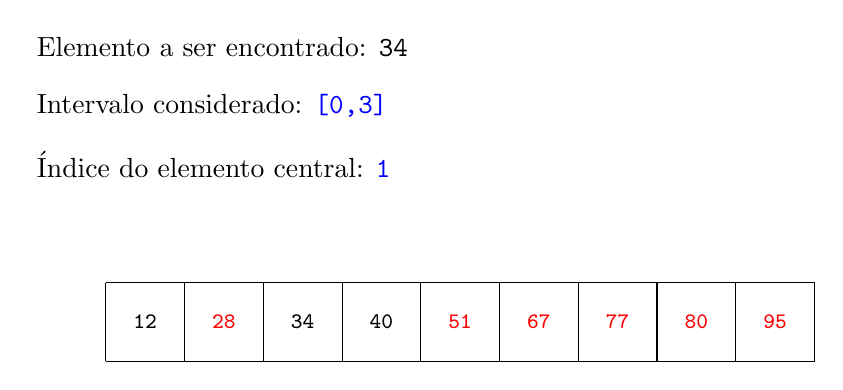
\begin{tikzpicture}
        \node[anchor=west] at (0, 4) {Elemento a ser encontrado: \texttt{34}};
        \node[anchor=west] at (0, 3.25) {Intervalo considerado: \texttt{\textcolor{blue}{[0,3]}}};
        \node[anchor=west] at (0, 2.5) {Índice do elemento central: \texttt{\textcolor{blue}{1}}};
        \draw (1,0) grid (10,1);

        \node at (1.5,0.5) {\footnotesize \texttt{12}};
        \node at (2.5,0.5) {\footnotesize \texttt{\textcolor{red}{28}}};
        \node at (3.5,0.5) {\footnotesize \texttt{\textcolor{black}{34}}};
        \node at (4.5,0.5) {\footnotesize \texttt{40}};
        \node at (5.5,0.5) {\footnotesize \texttt{\textcolor{red}{51}}};
        \node at (6.5,0.5) {\footnotesize \texttt{\textcolor{red}{67}}};
        \node at (7.5,0.5) {\footnotesize \texttt{\textcolor{red}{77}}};
        \node at (8.5,0.5) {\footnotesize \texttt{\textcolor{red}{80}}};
        \node at (9.5,0.5) {\footnotesize \texttt{\textcolor{red}{95}}};
    \end{tikzpicture}

\end{frame}

\begin{frame}[fragile]{Visualização da busca binária}

    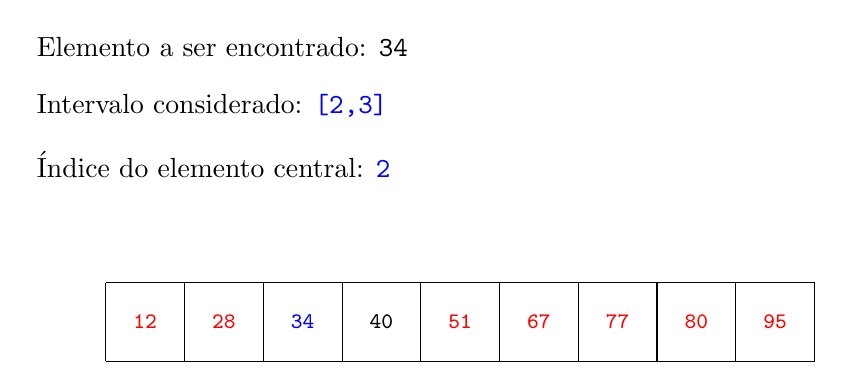
\begin{tikzpicture}
        \node[anchor=west] at (0, 4) {Elemento a ser encontrado: \texttt{34}};
        \node[anchor=west] at (0, 3.25) {Intervalo considerado: \texttt{\textcolor{blue}{[2,3]}}};
        \node[anchor=west] at (0, 2.5) {Índice do elemento central: \texttt{\textcolor{blue}{2}}};
        \draw (1,0) grid (10,1);

        \node at (1.5,0.5) {\footnotesize \texttt{\textcolor{red}{12}}};
        \node at (2.5,0.5) {\footnotesize \texttt{\textcolor{red}{28}}};
        \node at (3.5,0.5) {\footnotesize \texttt{\textcolor{blue}{34}}};
        \node at (4.5,0.5) {\footnotesize \texttt{\textcolor{black}{40}}};
        \node at (5.5,0.5) {\footnotesize \texttt{\textcolor{red}{51}}};
        \node at (6.5,0.5) {\footnotesize \texttt{\textcolor{red}{67}}};
        \node at (7.5,0.5) {\footnotesize \texttt{\textcolor{red}{77}}};
        \node at (8.5,0.5) {\footnotesize \texttt{\textcolor{red}{80}}};
        \node at (9.5,0.5) {\footnotesize \texttt{\textcolor{red}{95}}};
    \end{tikzpicture}

\end{frame}

\begin{frame}[fragile]{Exemplo de implementação da busca binária}
    \inputsnippet{cpp}{1}{21}{codes/bin_search.cpp}
\end{frame}

\begin{frame}[fragile]{Busca binária em C}

    \begin{itemize}
		\item A função \code{c}{bsearch()} da biblioteca \code{c}{stdlib.h} do C implementa a busca 
        binária

        \item A assinatura da função \code{c}{bsearch()} é
            \inputsyntax{c}{codes/bs.st}

        \item O parâmetro \code{cpp}{key} é um ponteiro para o valor a ser localizado no
            vetor \code{cpp}{base}

        \item O número de elementos do vetor \code{cpp}{base} é igual a \code{cpp}{nmemb}, e 
            cada um deste elementos ocupa \code{cpp}{size} \textit{bytes} em memória

        \item O parâmetro \code{cpp}{compar} é um ponteiro para uma função que recebe dois
            ponteiros e retorna negativo, zero ou positivo se o primeiro ponteiro aponta para
            um valor menor, igual ou maior do que o valor apontado pelo segundo ponteiro,
            respectivamente
    \end{itemize}

\end{frame}

\begin{frame}[fragile]{Busca binária em C++}

    \begin{itemize}
        \item A biblioteca \code{c++}{algorithm} do C++ traz três funções associadas à busca
            binária

        \item A função \code{c++}{binary_search()} retorna verdadeiro se o elemento a ser
        encontrado está no intervalo indicado
            \inputsyntax{c++}{codes/binary_search.st}

        \item As funções \code{c++}{lower_bound()} e \code{c++}{upper_bound()} retornam um iterador
        para o primeiro elemento maior ou igual a $x$, ou estritamente maior do que $x$, 
        respectivamente:
            \inputsyntax{c++}{codes/bounds.st}

    \end{itemize}

\end{frame}
\begin{frame}[fragile]{Exemplo de uso de busca binária em C e C++}
    \inputsnippet{c++}{1}{19}{codes/cbs.cpp}
\end{frame}

\begin{frame}[fragile]{Exemplo de uso de busca binária em C e C++}
    \inputsnippet{c++}{21}{43}{codes/cbs.cpp}
\end{frame}

\begin{frame}[fragile]{Método da bisecção}

    \begin{itemize}
        \item O método da bisecção utiliza a busca binária para identificar uma raiz de uma
            função $f(x)$ em um intervalo $(a, b)$

        \item Este método pode ser aplicado se $f(x)$ for contínua em $(a, b)$ e se
            $f(a)f(b) < 0$

        \item Isto significa que os valores de $f(x)$ nos extremos do intervalo tem sinais opostos

        \item Como $f(x)$ é continua no intervalo, partindo de $a$, ela tem que atravessar, ao
            menos uma vez, o eixo-$x$ para atingir o ponto $b$

        \item Seja $c$ um ponto tal que $f(c) = 0$

        \item O método da bisecção tenta localizar tal $c$, buscando, inicialmente, o elemento
            central do intervalo
    \end{itemize}

\end{frame}

\begin{frame}[fragile]{Método da bisecção}

    \begin{itemize}
        \item Caso este elemento não seja igual a $c$, isto significa que $f(m) \neq 0$

        \item A partir das relações entre $f(a), f(m)$ e $f(b)$, a busca continua ou no intervalo
            $(a, m)$ ou $(b, m)$

        \item O algoritmo deve ser interrompido quando $f(m) = 0$

        \item Porém, devido à aritmética de ponto flutuante, pode ser que ista condição jamais seja
            satisfeita

        \item Assim, pode-se adotar como critério de parada
        \begin{enumerate}
            \item um limiar $\varepsilon > 0$ e parar o algoritmo quando $f(m) < \varepsilon$, ou
            \item um número fixo $N$ de interações do algoritmo
        \end{enumerate}

        \item Em ambos casos, a complexidade do algoritmo é $O(\log(b - a))$
    \end{itemize}

\end{frame}

\begin{frame}[fragile]{Implementação da biseção com limiar}
    \inputsnippet{cpp}{1}{20}{codes/bisection.cpp}
\end{frame}

\begin{frame}[fragile]{Busca binária na resposta}

    \begin{itemize}
        \item Seja função $f(x)$ é monótona em um intervalo $[a, b]$

        \item Isto significa que $f(x)$ é não-decrescente ($f(x) \leq f(y)$, se $x\leq y$) ou
            não-crescente ($f(x) \geq f(y)$, se $x\leq y$) em $[a, b]$

        \item Assim, para uma sequência de valores $a\leq x_1 < x_2 < \ldots < x_N\leq b$, as 
            imagens $y_i = f(x_i)$ formarão uma sequência também monótona

        \item Deste modo, interpretanto os valores $x_i$ como os índices de um vetor cujos valores
            são $y_i$, é possível, por meio da busca binária, identificar um $x_0$ tal que
            $f(x_0) = y_0$ para um $y_0$ escolhido

        \item Esta técnica, denominada busca binária na resposta, é útil quando $f(x)$ é uma função
            monótona que é difícil de computar
            ou que representa um processo elaborado, e se deseja encontrar um valor $x_0$ que
            atenda uma série de pré-requisitos ou condições
    \end{itemize}

\end{frame}

\begin{frame}[fragile]{Exemplo de busca binária na resposta: Triângulo de Pascal}

    \begin{itemize}
        \item Considere o seguinte problema: dado $M \leq 10^{18}$, determine o menor $N$ tal que
            a $N$-ésima linha do Triângulo de Pascal contenha ao menos um coeficiente maior ou
            igual a $M$

        \item O Triângulo de Pascal é formado pela linha 0, que contém apenas o número 1, a linha
            1, com dois números 1, e as demais linhas começam e terminam com 1, e os elementos
            intermediários são formados pela soma dos dois elementos imediatamente acima

            \input{pascal}

    \end{itemize}

\end{frame}

\begin{frame}[fragile]{Exemplo de busca binária na resposta: Triângulo de Pascal}

    \begin{itemize}
        \item De fato, o $i$-ésimo coeficienta da linha $n$ é dado por
        $$
            C(n, i) = \binom{n}{i} = \frac{n!}{(n - i)!i!}
        $$

        \item Observe que o maior coeficiente da linha $n$ ocupa a posição central

        \item Assim, se $c_k$ é o coeficiente que ocupa a posição central da $k$-ésima linha, 
            a sequência $\{ c_1, c_2, \ldots, c_N\}$ é monótona, de modo que o problema pode ser
            resolvido por meio de busca binária na resposta

        \item Por inspeção, $c_0 = 1$ e $c_{64} = 1832624140942590534 > 10^{18}$

        \item Assim, basta realizar a busca no intervalo $[0, 64]$

        \item Como cada coeficiente pode ser computado em $O(N)$, a complexidade da solução será
            $O(N\log I)$, onde $I$ é o tamanho do intervalo de busca
    \end{itemize}

\end{frame}

\begin{frame}[fragile]{Implementação do exemplo em Python}
    \inputsnippet{python}{1}{20}{codes/pascal.py}
\end{frame}
